\thispagestyle{empty}
\setcounter{figure}{0}
\chapter{Spektrogramy} \label{appendix:spectrogram}
\pagenumbering{arabic}
\renewcommand*{\thepage}{D-\arabic{page}}
     
\begin{figure}[h]
	\centering
    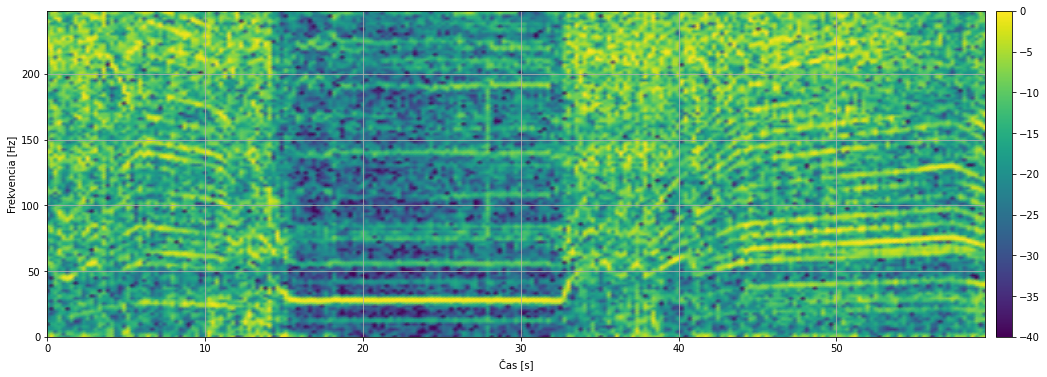
\includegraphics[width=\textwidth]{figures/verification/L83-dataset-spectrum.png}
	\caption{Spektrogram záznamu z vozidla \emph{L83\_4940\_Alexyho\_Svantnerova.csv}}
\end{figure}

\begin{figure}[h]
	\centering
    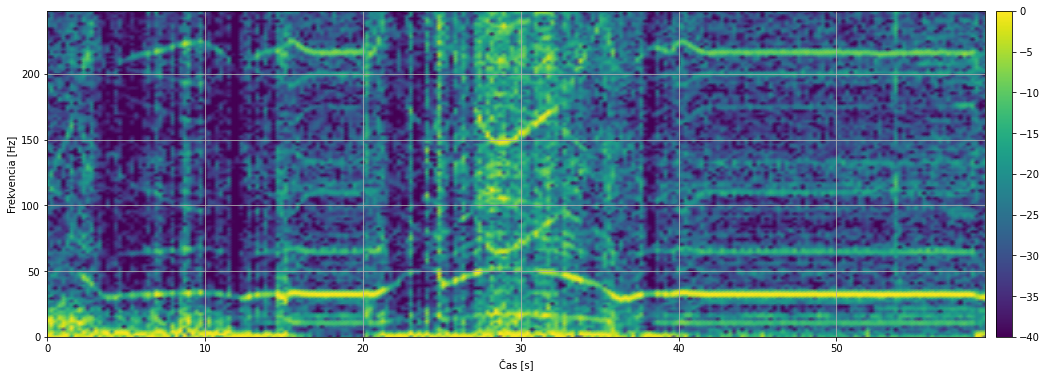
\includegraphics[width=\textwidth]{figures/verification/L35-dataset-spectrum.png}
    \caption{Spektrogram záznamu z vozidla \emph{L35\_1915\_Borska\_Zaluhy.csv}}
\end{figure}

Detekcia udalostí pri vzorkovacej frekvencii 500 Hz, dĺžkou FFT 256 bodov,
$t_{min} = 10$ a $t_{\Delta} = 4$ na datasete \emph{L35\_1915\_Borska\_Zaluhy.csv}:

\begin{figure}[h]
	\centering
    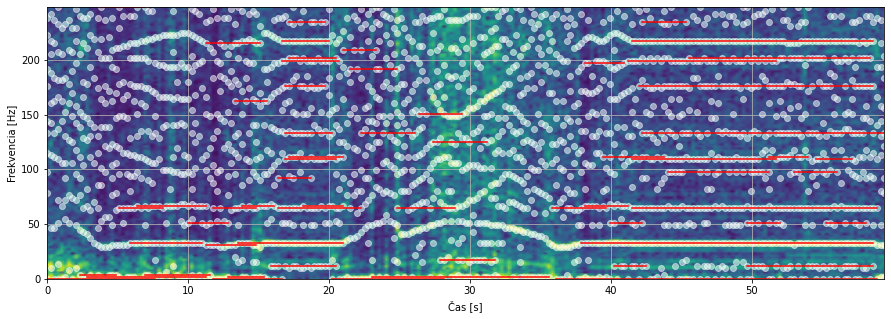
\includegraphics[width=\textwidth]{figures/verification/L35-dataset-A1.png}
    \caption{Algoritmus č.1: $k = 5$, $\epsilon = 0$, $h_{rel} = 8$}
\end{figure}

\begin{figure}[h]
	\centering
    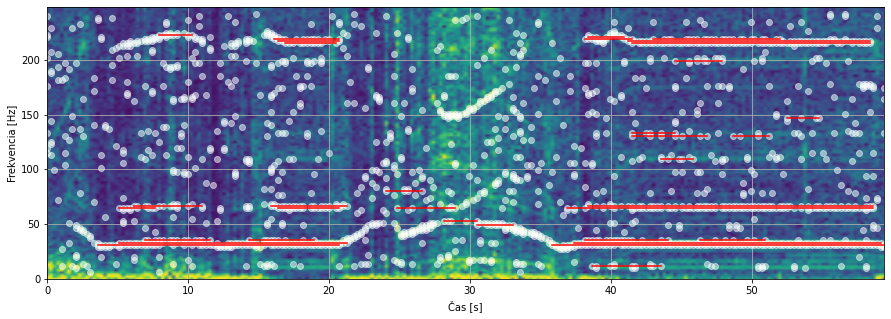
\includegraphics[width=\textwidth]{figures/verification/L35-dataset-A2.png}
    \caption{Algoritmus č.2: $k = 3$, $s = 7$}
\end{figure}

\begin{figure}[h]
	\centering
    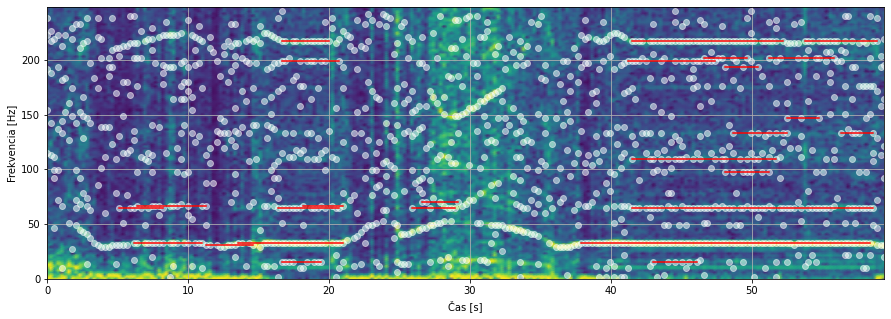
\includegraphics[width=\textwidth]{figures/verification/L35-dataset-A3.png}
    \caption{Algoritmus č.3: $t = 8$, $h = 1$, $p = 5$, $i = 0$}
\end{figure}


\thispagestyle{empty}
\setcounter{figure}{0}
\chapter{Obsah digitálneho média}
\pagenumbering{arabic}
\renewcommand*{\thepage}{E-\arabic{page}}
\par Evidenčné číslo práce v informačnom systéme: \RegNo
\par Obsah digitálnej časti práce (archív ZIP):
\par Názov odovzdaného archívu: BP\_MiroslavHajek.zip

\begin{itemize}[noitemsep]
\item[\textbf{>}] \textbf{firmware} - Zdrojový kód firmvéru senzorovej jednotky
	\begin{itemize}
	\item[\textbf{>}] \textbf{esp-dsp} - ESP DSP Library - knižnica na optimalizáciu spracovania signálov na ESP32.
	\item[\textbf{>}] \textbf{esp-idf} - Espressif IoT Development Framework - SDK pre hardvér ESP32.
	\item[\textbf{>}] \textbf{mpack} - MPack knižnica enkódera a dekódera MessagePack serializačného formátu.
	\item[\textbf{>}] \textbf{vibration-analyzer} - Samotná implementácia aplikačnej logiky.
		\begin{itemize}
		\item[\textbf{>}] \textbf{conf} - Konfiguračné súbory pre OpenLog (\emph{config.txt}), MQTT broker  (\emph{mosquitto.conf})
		a na zostavenie dokumentácie cez Doxygen (\emph{doxygen.conf}).
		\item[\textbf{>}] \textbf{docs} - Doxygen dokumentácia. Úvodná stránka je \emph{index.html}.
		\item[\textbf{>}] \textbf{main}
			\begin{itemize}
			\item[\textbf{>}] \textbf{include} - Hlavičkové súbory \emph{.h} aplikácie.
			\item[\textbf{>}] \textbf{src} - Zdrojové súbory \emph{.c} aplikácie.
			\end{itemize}
		\item[\textbf{>}] \textbf{tests} - Jednotkové testy na kontrolu najdôležitejšej funkcionality a validujúce konzistenciu
		medzi Python a C implementáciou algoritmov: \emph{test\_events.c} (test prúdového algoritmu nájdenia zmeny frekvencií),
		\emph{test\_peaks.c} (test klasifikátorov špičiek), \emph{test\_config.py} (test vzdialenej konfigurácie zariadenia).
		Nástroj na interaktívny vzdialený prístup k IoT jednotke \emph{config\_tool.py}.
		\end{itemize}
	\end{itemize}
\item[\textbf{>}] \textbf{measurements} - Analýza dátových sád a generovanie syntetických signálov v notebookoch \emph{.ipynb}.
	\begin{itemize}
	\item[\textbf{>}] \textbf{datasets} - Vibračné záznamy z vozidiel verejnej dopravy.
	\item[\textbf{>}] \textbf{experiments} - Pôvodné monitorovacie výpisy z experimentov slúžiace ako poklad na overenie riešenia.
		\begin{itemize}
			\item[\textbf{>}] \textbf{accuracies} - Úspešnosti klasifikácie na syntetickom spektrálnom profile. Súbor \emph{results.txt}.
			vychádza z analýzy v \emph{VibrationProcessingAlgorithms.ipynb}, do tabuľkovej podoby sa dostal v \emph{results-table.csv}.
			\item[\textbf{>}] \textbf{execution-algorithms} - Časy vykonávania jednotlivých algoritmov.
			\item[\textbf{>}] \textbf{execution-pipeline} - Časy vykonávania celej dátovej pipeline.
			\item[\textbf{>}] \textbf{memory-usage} - Spotreba flash pamäte.
			\item[\textbf{>}] \textbf{network} - Odchytená sieťová komunikácie z MQTT broker v \emph{.pcap} súboroch.
		\end{itemize}
	\item[\textbf{>}] \textbf{signals} - Užitočné funkcie ku prieskumnej analýze, vizualizácii a tvorbe modelov v Jupyter notebookoch.	
	\end{itemize}
\end{itemize}
